%% LyX 1.6.1 created this file.  For more info, see http://www.lyx.org/.
%% Do not edit unless you really know what you are doing.
\documentclass[10pt,italian,sans]{beamer}
\usepackage[3D]{movie15}
\usepackage{babel}
\usepackage{ae,aecompl}
\usepackage[T1]{fontenc}
\usepackage[latin9]{inputenc}
\setcounter{tocdepth}{2}
\usepackage{amsmath}
\usepackage{graphicx}
\usepackage{amssymb}
\usepackage{verbatim}
%\includeonlyframes{current_frame}

\makeatletter
%%%%%%%%%%%%%%%%%%%%%%%%%%%%%% Textclass specific LaTeX commands.
 % this default might be overridden by plain title style
 \newcommand\makebeamertitle{\frame{\maketitle}}%
 \AtBeginDocument{
   \let\origtableofcontents=\tableofcontents
   \def\tableofcontents{\@ifnextchar[{\origtableofcontents}{\gobbletableofcontents}}
   \def\gobbletableofcontents#1{\origtableofcontents}
 }
\newcommand\itemat[2]{\only<{#1}>{\begin{enumerate} \setcounter{enumi}{#1} \item{#2} \end{enumerate}}}

\renewcommand\emph[2]{\textcolor{#1}{\textbf{{#2}}}}

\newcommand\lyxframe[1]{\begin{frame}[fragile]{#1}}
    \setcounter{MaxMatrixCols}{15}


%%%%%%%%%%%%%%%%%%%%%%%%%%%%%% User specified LaTeX commands.
\usepackage{xcolor}
\usepackage{multicol}

%
%\usetheme{Darmstadt}
\usetheme{Frankfurt}
%+++spartano, ok

%\usetheme{Madrid}
%+++ senza boxes, ma carino
%\usetheme{Pittsburgh}
%+ square
%\usetheme{Rochester}
%\usetheme{Singapore}
%super tipico
%\usetheme{Warsaw}

%\usepackage{pstcol,pst-node,pst-tree}
% or ...
%\usecolortheme{albatross}
%\usecolortheme{beaver}
%\usecolortheme{beetle}
%arancione,vivace
%\usecolortheme{crane}

%identico al default
%\usecolortheme{dolphin}
%come il default, piu delicato
%\usecolortheme{rose}
%tutto grigio....
%\usecolortheme{seagull}
% come default, header piu chiaro 
%\usecolortheme{seahorse}
%tutto uguale, header arancione!!!
%\usecolortheme{wolverine}

%\useoutertheme{infolines}
\useoutertheme[subsection=false]{miniframes}
%\useoutertheme{shadow}
%carino
%\useoutertheme{smoothbars}
%\useoutertheme{split}
%\useoutertheme{tree}
%\useoutertheme{default}


%\usepackage{euler}
%

\setbeamercovered{transparent=15}
\setbeamertemplate{navigation symbols}{}
\useinnertheme{circles}
% or whatever (possibly just delete it)
%\usefonttheme{structuresmallcapsserif}
\setbeamerfont{headline}{size=\footnotesize}

\makeatother


\begin{document}

\title{Sviluppi Teorici e Applicativi delle Metriche Entropiche di Rohlin}




\author{Dawid Crivelli\\
%\includegraphics[height=0.4\textwidth]{images/pfoldfig.png}
}

\date{26 Aprile 2012}

\makebeamertitle


\begin{frame}{Sommario}
\tableofcontents{}
\end{frame}

\section{Distanze Entropiche}

\begin{frame}{Proteine dell'influenza H3N2}

\begin{columns}
\column{0.5\textwidth}
\begin{itemize}
\item proteine come stringhe 
\item approccio \textit{black box}
\item sequenze lunghe 566
\item alfabeto di 24 lettere
\item solo 10\% mutazioni
\item \emph{black}{antigenic drift}
\end{itemize}

\column{0.5\textwidth}
\includegraphics[height=0.5\textheight]{../immagini/swine-flu}
%\center{\small{Struttura del virus}}
\end{columns}
\medskip{}
Sequenze a confronto:
\medskip{}
\includegraphics[width=1\textwidth]{seq_lines2}

\end{frame}



\begin{frame}[fragile]
\frametitle{Hamming \`e poco adatto}
\begin{columns}[b]
\column{0.65\textwidth}
\only<1>{\begin{semiverbatim} 
A=\{GHHAVPNGTLVKTITTGRICGDPHCDGFQNKEW\}

B=\{GHHAVPNGTIVKTITTGEICGDPQCDGFQNKKW\}
\end{semiverbatim}}
\only<2->{\begin{semiverbatim} 
A=\{GHHAVPNGT\textbf{{\color{red}{L}}}VKTITTG\emph{red}{R}ICGDP\emph{red}{H}CDGFQNK\emph{red}{E}W\}

B=\{GHHAVPNGT\emph{red}{I}VKTITTG\emph{red}{E}ICGDP\emph{red}{Q}CDGFQNK\emph{red}{K}W\}
\end{semiverbatim}}
\column{0.35\textwidth}
$d_H(A,B)$= \#differenze 
\visible<2->{$d_H(A,B)=4$}
\end{columns}
\bigskip{}

\begin{columns}
\column{0.65\textwidth}
\visible<3->{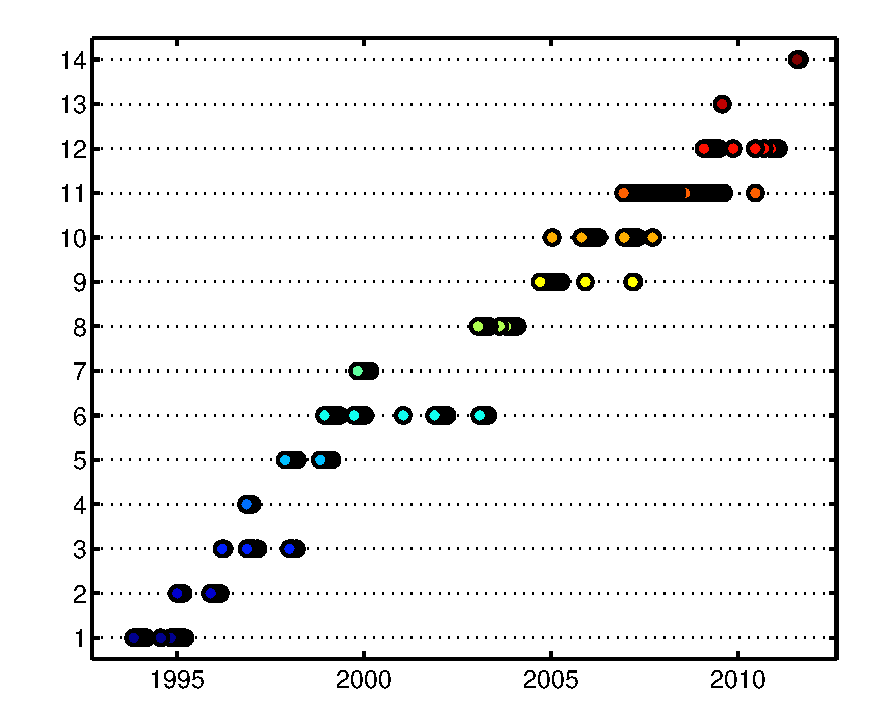
\includegraphics[width=0.9\textwidth]{../grafici/clusters_hamming2}}

\column{0.35\textwidth}
\visible<3->{
\begin{block}{Antigenic drift}
$d_H \propto t$
\end{block}
}
\end{columns}
\end{frame}

\lyxframe{Distanza di Rohlin}
Distanza non tra configurazioni, ma tra \emph{black}{partizioni}\\
\bigskip{}
Requisiti:
\begin{itemize}
\item uno spazio di probabilit\`a: $(\mathbf{M},\sigma,\mu)$ 
\item un criterio per partizionare (relazione di equivalenza)
\item usiamo $\mathbf{M}$ discreto, $\mu$ \`e banale
\end{itemize}

\bigskip{}
Applicabile a molte strutture diverse:\\
\medskip{}
\begin{center}
\includegraphics[width=0.3\textwidth]{seq_lines3}\hfill{}
\includegraphics[width=0.3\textwidth,height=0.3\textheight]{reticolo-semplice}\hfill{}
\includegraphics[width=0.3\textwidth,height=0.3\textheight]{sierpinski}
\end{center}

\end{frame}
\lyxframe{Complessit\`a di una partizione}
\begin{comment}
Ad ogni partizione corrispondono configurazioni diverse:\\
\begin{center}
{\tt\{
\colorbox{red}{AAAA}
\colorbox{green}{BB}
\colorbox{blue}{CCC}
\colorbox{red}{AAAA}
\}}\\
{\tt\{
\colorbox{red}{BBBB}
\colorbox{green}{ZZ}
\colorbox{blue}{AAA}
\colorbox{red}{FFFF}
\}}
\end{center}
\end{comment}
Partizione $\Longleftrightarrow$ scomposizione in \emph{black}{atomi} disgiunti di \textit{misura} $\mu(A_k)$
\bigskip{}

Rappresentazione associando ad ogni sito un'etichetta (atomo):\\
\[\mathrm{A}=\{\underbrace{(1,2,3,4)}_{A_1},\underbrace{(5,6)}_{A_2},\underbrace{(7,8,9)}_{A_3},\underbrace{(10,11,12,13)}_{A_4}\}\]
\medskip{}
\[\mathrm{A}=
\begin{bmatrix}
 1 &  2 &  3 &  4 &  5 &  6 &  7 &  8 &  9 & 10 & 11 & 12 & 13 \\
 \colorbox{red}{1} &  \colorbox{red}{1} &  \colorbox{red}{1} &  \colorbox{red}{1} &  \colorbox{green}{2} &  \colorbox{green}{2} &  \colorbox{blue}{3} &  \colorbox{blue}{3} &  \colorbox{blue}{3} &  \colorbox{orange}{4} &  \colorbox{orange}{4} &  \colorbox{orange}{4} &  \colorbox{orange}{4} \\
\end{bmatrix}
\]

\bigskip{}

\emph{black}{Entropia di Shannon}: misura della complessit\`a di una partizione
\[H(A)=\sum_k^n \mu(A_k) \log\left(\mu(A_k)\right)\]

\begin{center}
\begin{tabular}{ll}
H=$\log(n)$ (max) & $\Leftrightarrow$ partizione con n atomi equivalenti\\
H=0 (min) & $\Leftrightarrow$ partizione banale $\nu$
\end{tabular}
\end{center}
\end{frame}

\lyxframe{Partizionamento}
\center{un partizione \`e una relazione di equivalenza}, $i \sim j \Longleftrightarrow i,j \in A_k$

\bigskip{}
\begin{overprint}
\only<1>{\center{\includegraphics[height=0.5\textheight]{reticolo-semplice2}}}

\only<2>{\center{\includegraphics[height=0.5\textheight]{reticolo-bond}}}
\end{overprint}
relazione locale(tra vicini) => partizione globale\\
	=> colorazione di grafi, algoritmo Hoshen-Kopelman $\mathcal{O} (N\log(N))$

\end{frame}


\lyxframe{Prodotti tra partizioni}
Partizione prodotto $\gamma = \alpha \vee \beta$

\begin{columns}
\column{0.45\textwidth}
\begin{itemize}
\item propriet\`a associativa
\item elemento neutro $\nu$
\item ogni partizione \`e scrivibile come prodotto
\item idempotente \[\alpha \vee \alpha = \alpha\]
\item l'entropia del prodotto \`e sempre maggiore \[H(\alpha \vee \beta)\geq H(\alpha),\; \forall \beta\]
\end{itemize}
\column{0.55\textwidth}
\center{\includegraphics[height=0.6\textheight]{prodotto}}\null
\end{columns}
\end{frame}
\lyxframe{Distanza di Rohlin}

Distanza tra partizioni, tramite l'entropia del prodotto:
\[d_R(\alpha,\beta) = 2\,H(\alpha \vee \beta) - H(\alpha) - H(\beta)\]

Partizioni simili hanno piccola distanza:
\medskip{}
\includegraphics[height=0.2\textheight]{distanze}

\bigskip{}

Cosa fare per partizioni molto diverse e frammentate?
\medskip{}
\includegraphics[height=0.2\textheight]{distanze2}

\end{frame}
\lyxframe{Intersezione tra partizioni}
Definiamo $\sigma = \alpha \wedge \beta$, la partizione \emph{black}{comune}

\end{frame}
\lyxframe{Riduzione e amplificazione della distanza}


\end{frame}


\lyxframe{Definizione topologica della distanza}


\end{frame}
\end{document}

\lyxframe{Clustering di sequenze}


\end{frame}\lyxframe{La riduzione lineare funziona meglio}


\end{frame}\section{Sistemi magnetici}


\end{frame}\lyxframe{Sequenze lineari di spin (Ising 1D)}


\end{frame}\lyxframe{Clusters di spin $\Longleftrightarrow$ Clusters di link}


\end{frame}\lyxframe{Lunghezza di correlazione tra partizioni}


\end{frame}\lyxframe{Variazione in temperatura}


\end{frame}\lyxframe{Tipi di disordine}


\end{frame}\lyxframe{Ising 2D, reticolo quadrato}
\end{frame}

\end{document}

\section{Distanze}
\subsection{Definizioni}

\begin{frame}{Dov'\`e applicabile?}

Su ogni spazio di probabilit\`a ($\mathbf{M},\;\sigma,\;\mu$). 

Esempi: \textbf{\uncover<2>{\textcolor{green!50!black}{Sequenze Lineari }}\uncover<3>{\textcolor{red}{Reticoli Regolari }}\uncover<4>{\textcolor{blue}{Grafi }}}\\
\begin{overlayarea}{1\textwidth}{0.7\textheight}

\only<1>{ 

}

\only<2>{
\begin{block}{Terziaria: Accurata rappresentazione 3D della molecola}
%\center{\includegraphics[c,width=0.8\textwidth]{images/struttura_terziaria}}
\end{block}
}

\only<3>{
\begin{block}{Cosa ci dice:}
\begin{enumerate}
\item Molte rappresentazioni equivalenti, ad es la permutazione
\item Rappresenta i contatti tra le basi
\end{enumerate}
\end{block}
\begin{alertblock}{Permutazione}
\[
\sigma=\left[\begin{smallmatrix}
 1 &  2 &  3 &  4 &  5 &  6 &  7 &  8 &  9 & 10 & 11 & 12 & 13 & 14 & 15 & 16 \\
 A &  A &  A &  G &  G &  U &  C &  A &  U &  U &  C &  G &  G &  G &  G &  G \\
 | &  | &  | &  | &  | &  | &  | &  | &  | &  | &  | &  | &  | &  | &  | &  | \\
 U &  U &  U &  C &  C &  G &  G &  U &  G &  A &  G &  G &  G &  G &  G &  C \\
26 & 25 & 24 & 23 & 22 & 21 & 20 & 19 & 18 & 17 & 16 & 12 & 13 & 14 & 15 & 11 
\end{smallmatrix}\right]
\]
\end{alertblock}
}
\only<4>{ 
%\includegraphics[c,height=0.8\textheight]{images/1vp0_A_bi.png}
}

\end{overlayarea}
\end{frame}



\subsection{Differenze tra modello e RNA reale}
\begin{frame}{Differenze tra RNA vero e modello}

%
\begin{figure}
\includegraphics<1>[width=1\textwidth]{images/non_stand1.png}
\includegraphics<2->[width=1\textwidth]{images/non_stand2.png}
\end{figure}

\begin{columns}
\column{0.5\textwidth}
\uncover<2->{
\begin{itemize}[<alert@+(+1)>]
\item Legami tra basi uguali e non canonici
\item Nessun vincolo di vicinanza (anzi, stacking)
\end{itemize}
}
\column{0.5\textwidth}
\begin{overprint}
\begin{exampleblock}<2>{Esempi:}
{A-A, G-G, C-A, U-C}
\end{exampleblock}
\end{overprint}
\end{columns}


\end{frame}

\subsection{Criteri per la scelta dei legami}
\begin{frame}[fragile]   
\frametitle{Criteri per la scelta dei legami}
\begin{columns}
\column{0.64\textwidth}
{\small\begin{semiverbatim} 
B:   1 G-C  2876 B: +/+ cis    XIX
B:   3 U-A  2874 B: -/- cis    XX
\invisible<10->{\alert<9>{B:   4 A-U     6 B: -/- cis    XX}}
\invisible<3->{\alert<2>{B:   7 G-C    22 A: +/+ cis    XIX}}
\invisible<4->{\alert<3>{B:   8 A-A  2608 B: W/H tran   V}}
B:  17 G-C   533 B: +/+ cis    XIX
\invisible<6->{\alert<5>{B:  17 G-U   534 B: stacked}}
B:  18 U-A   532 B: -/- cis    XX
\invisible<5->{\alert<4>{B: 177 U-G   227 B: W/W tran   XXVII}}
\invisible<6->{\alert<5>{B: 727 U-A   731 B: S/W cis    n/a}}
\invisible<4->{\alert<3>{B:  21 A-G   528 B: W/W cis    VIII}}
\invisible<9->{\alert<8>{B:  74 G-C   201 B: +/+ cis    XIX}}
\alert<8>{B:  74 G-U   110 B: W/W cis    XXVIII}
B:  78 C-G   105 B: +/+ cis    XIX
\invisible<3->{\alert<2>{B:  79 G-P    88 B: W/S tran   n/a}}
B:  80 A-U   103 B: -/- cis    XX
\invisible<7->{\alert<6>{B: 211 U-A   443 B: W/W tran   XXI}}
\alert<7>{A: 459 A-U   472 A: -/- cis    XX}
\invisible<8->{\alert<7>{A: 459 A-U   473 A: -/- cis    XX}}
\end{semiverbatim}
}
\column{0.36\textwidth}
{\small
\begin{block}{Rimuoviamo i legami:}
\begin{enumerate}[<+(+1)->]
\item {tra oggetti diversi} %2
\item {basi incompatibili} %3
\item {legami G-U non wobble-pair} %4
\item {lati non Watson-Crick} %5
\item {lati Watson-Crick trans} %7
\item {legami ambigui} %8
\item {legami meno importanti} %9
\item {basi troppo vicine} %9
\end{enumerate}
\end{block}
\visible<+(+1)->{\begin{alertblock}{in media 37\% rimossi!}{pi\`u del previsto}\end{alertblock}}
}
\end{columns}
\end{frame}

\section{Pseudonodi}
\subsection{Grafici (non)planari}
\begin{frame}{Grafi}
\begin{overprint}
\only<1>{
\begin{block}{Planare}
\begin{itemize}
\item Si rappresenta su un piano
\item Semplici regole di ricorrenza
\item Minimizzazione $\mathcal{O}(n^{2-3})$
\end{itemize}
\end{block}
}
\only<2->{
\begin{alertblock}{Non planare}
\begin{itemize}[<+(+2)->]
\item Su un piano si vedono intersezioni
\item \emph{blue}{Pseudonodi}: I gruppi di legami che incrociano altri
\item Nonplanare = Multiplamente-planare
\item Minimizzazione generale NP-hard
\end{itemize}
\end{alertblock}
}
\end{overprint}
\bigskip{}
\begin{overlayarea}{1\textwidth}{0.4\textheight}
\center{
\includegraphics<1>[height=0.35\textheight]{images/genus_crescente1.png}
\includegraphics<2-3>[height=0.35\textheight]{images/genus_crescente2.png}
\includegraphics<4->[height=0.35\textheight]{images/genus_crescente3.png}
}
\end{overlayarea}
\end{frame}

\subsection{L'Invariante di Euler}
\begin{frame}
\frametitle{L'invariante di Euler}

\center{{\Large  $\chi=\alert<3>{c_0} \alert<4>{-c_1} \alert<5>{+ c_2} $}}

\medskip{}
\begin{block}{Come calcolarlo}
\begin{enumerate}[<+(+1)->]
\item Passaggio ai doppi legami
\item Numero dei punti - le doppie basi
\item Numero degli archi
\item Numero superfici colorate
\item Relazione tra archi e superfici indipendenti
\end{enumerate}
\end{block}

\medskip{}

\begin{overlayarea}{1\textwidth}{0.3\textheight}
\center{
\includegraphics<1>[height=0.28\textheight]{images/doppio1.png}
\includegraphics<2>[height=0.28\textheight]{images/doppio2.png}
\includegraphics<3>[height=0.28\textheight]{images/doppio3.png}
\includegraphics<4>[height=0.28\textheight]{images/doppio4.png}
\includegraphics<5->[height=0.28\textheight]{images/doppio5.png}
}
\end{overlayarea}
\end{frame}

\begin{frame}{$\chi$ ed il genus}
La superficie di embedding ha  \emph{purple}{genus minimale} g

\bigskip{}
\includegraphics[height=0.35\textheight]{images/toro1.png}
\includegraphics[height=0.35\textheight]{images/toro2.png}

\bigskip{}
\begin{overprint}
\uncover<2->{
\emph{green!50!black}{Teorema di Euler}: 
Una superficie orientabile ha \emph{red}{genus} $\displaystyle g=\frac{2-\chi}{2}$}\\
\bigskip{}
\uncover<3->{
Nel nostro caso, i colori non sono dipendenti, dipendono dal \emph{blue}{numero di cammini indipendenti $n_{loop}$}, rispetto al totale $n_{archi}$\\

\[g=\frac{n_{archi}-n_{loop}}{2}\]}
\end{overprint}
\end{frame}

\subsection{Distribuzione sperimentale del genus}
\begin{frame}
\frametitle{Risultati statistiche sui genus}
\framesubtitle{Analisi di 800 molecole da PDB e NDB}
\includegraphics[t,height=0.6\textheight]{/home/fake/tesi/images/distr_genus}

\bigskip{}

Il genus di un polimero libero tende a $\displaystyle  \frac{\operatorname{L}}{4}$, dell'RNA circa $\displaystyle\frac{\operatorname{L}}{300}$.

\bigskip{}

\emph{green!50!black}{Il genus pesa}, con un \emph{red!75!black}{potenziale} coniugato: F = E -TS -\textcolor{red!75!black}{$\boldsymbol\mu$}\emph{green!50!black}{g}
\end{frame}


\section{Cell}
\subsection{Overview}
\begin{frame}
\frametitle{Overview}
\includegraphics[t,height=0.85\textheight]{/home/fake/tesi/images/cell-chip}

\end{frame}

\subsection{Spu}
\begin{frame}
\frametitle{Operazioni vettoriali}
\begin{overlayarea}{1\textwidth}{0.8\textheight}
\begin{itemize}%[<+->]
\item{Operazioni su pi\`u elementi contemporaneamente\\
\center{\includegraphics[t,height=0.30\textheight]{/home/fake/tesi/images/spu_scalar_slots}}}
\only<2->{\item{Si scambiano velocemente posizione agli elementi dei vettori\\
\center{\includegraphics[t,height=0.35\textheight]{/home/fake/tesi/images/spu_shuffle}}}}
\end{itemize}
\end{overlayarea}
\end{frame}

\begin{frame}[fragile]
\frametitle{Lettura di scalari}
\begin{overlayarea}{1\textwidth}{0.8\textheight}
\begin{itemize}%[<+->]
\item<+->{La vettorialit\`a si paga sugli scalari -- $c[2]+=5$ diventa:\\
\scriptsize{
\begin{semiverbatim}
\alert<+>{0D  90                        il      \$4,2	}
\alert<+>{1D  9012                      cbd     \$6,2(\$3)       }
\alert<.>{0D   01                       ai      \$11,\$3,15    }  
\alert<+>{1D   -123456                  lqx     \$10,\$3,\$4     }
\alert<.>{1        -----7890              rotqby  \$7,\$10,\$11  }  
\textcolor<+>{blue}{0             ---12            ahi     \$5,\$7,5       }
\alert<+>{1                -3456        shufb   \$2,\$5,\$10,\$6   }
\alert<.>{1                   ---789012  stqx    \$2,\$3,\$4      }
\end{semiverbatim}
}
}
\only<+->{\item{Si scambiano velocemente posizione agli elementi dei vettori\\
\center{\includegraphics[t,height=0.35\textheight]{/home/fake/tesi/images/spu_shuffle}}}}
\end{itemize}
\end{overlayarea}
\end{frame}

\subsection{Evitare i conti scalari}
\begin{frame}
\frametitle{Il fondamento dei nostri algoritmi}
\framesubtitle{Lookup veloce di tabelle}
\center{\includegraphics[width=0.9\textwidth]{/home/fake/tesi/images/spu_lookup2}}
\begin{overprint}
\begin{block}<2->{Lettura di un vettore su \only<-2>{128}\only<3>{256}\only<4>{512} byte}
\only<-2>{
\begin{tabular}{lll}
Scalare & \colorbox{red}{\textcolor{red}{mmmmmmm}} & 70 cicli\\
Vettoriale & \colorbox{green!60!fg}{\textcolor{green!60!fg}{mm}} & 20 cicli
\end{tabular}
}
\only<3>{
\begin{tabular}{lll}
Scalare & \colorbox{red}{\textcolor{red}{mmmmmmm}} & 70 cicli\\
Vettoriale & \colorbox{green!60!fg}{\textcolor{green!60!fg}{mmmm}} & 40 cicli
\end{tabular}
}
\only<4>{
\begin{tabular}{lll}
Scalare & \colorbox{green!60!fg}{\textcolor{green!60!fg}{mmmmmmm}} & 70 cicli\\
Vettoriale & \colorbox{red}{\textcolor{red}{mmmmmmmm}} & 80 cicli
\end{tabular}
}
\end{block}
\end{overprint}
\end{frame}


\begin{frame}
\frametitle{Il fondamento dei nostri algoritmi}
\framesubtitle{Lookup veloce di tabelle}
\center{\includegraphics[width=0.9\textwidth]{/home/fake/tesi/images/spu_lookup2}}
\begin{overprint}
\begin{alertblock}{Operazioni scalari con 16 byte}
\begin{tabular}{lll}
\only<-1>{Lettura con lookup & \colorbox{green!60!fg}{\textcolor{green!60!fg}{mm}} & 40 cicli\\
Scrittura & \colorbox{red}{\textcolor{red}{mmmmmmmmmmmm}} & 240 cicli%
}\only<2>{%
Lettura scalare & \colorbox{green!60!fg}{\textcolor{green!60!fg}{mmmr}} & 70 cicli\\
Scrittura & \colorbox{red}{\textcolor{red}{mmmmmmmmmmmm}} & 240 cicli}%
\end{tabular}
\end{alertblock}
\end{overprint}
\end{frame}

%
%\begin{frame}
%\frametitle{Scomposizione scalare in loops}
%Animazione:\\
%\bigskip{}
%\animate<1-50>
%\includegraphics<1>[width=0.6\textwidth]{anim/coloranim01.png}
%\includegraphics<2>[width=0.6\textwidth]{anim/coloranim02.png}
%\includegraphics<3>[width=0.6\textwidth]{anim/coloranim03.png}
%\includegraphics<4>[width=0.6\textwidth]{anim/coloranim04.png}
%\includegraphics<5>[width=0.6\textwidth]{anim/coloranim05.png}
%\includegraphics<6>[width=0.6\textwidth]{anim/coloranim06.png}
%\includegraphics<7>[width=0.6\textwidth]{anim/coloranim07.png}
%\includegraphics<8>[width=0.6\textwidth]{anim/coloranim08.png}
%\includegraphics<9>[width=0.6\textwidth]{anim/coloranim09.png}
%\includegraphics<10>[width=0.6\textwidth]{anim/coloranim10.png}
%\includegraphics<11>[width=0.6\textwidth]{anim/coloranim11.png}
%\includegraphics<12>[width=0.6\textwidth]{anim/coloranim12.png}
%\includegraphics<13>[width=0.6\textwidth]{anim/coloranim13.png}
%\includegraphics<14>[width=0.6\textwidth]{anim/coloranim14.png}
%\includegraphics<15>[width=0.6\textwidth]{anim/coloranim15.png}
%\includegraphics<16>[width=0.6\textwidth]{anim/coloranim16.png}
%\includegraphics<17>[width=0.6\textwidth]{anim/coloranim17.png}
%\includegraphics<18>[width=0.6\textwidth]{anim/coloranim18.png}
%\includegraphics<19>[width=0.6\textwidth]{anim/coloranim19.png}
%\includegraphics<20>[width=0.6\textwidth]{anim/coloranim20.png}
%\includegraphics<21>[width=0.6\textwidth]{anim/coloranim21.png}
%\includegraphics<22>[width=0.6\textwidth]{anim/coloranim22.png}
%\includegraphics<23>[width=0.6\textwidth]{anim/coloranim23.png}
%\includegraphics<24>[width=0.6\textwidth]{anim/coloranim24.png}
%\includegraphics<25>[width=0.6\textwidth]{anim/coloranim25.png}
%\includegraphics<26>[width=0.6\textwidth]{anim/coloranim26.png}
%\includegraphics<27>[width=0.6\textwidth]{anim/coloranim27.png}
%\includegraphics<28>[width=0.6\textwidth]{anim/coloranim28.png}
%\includegraphics<29>[width=0.6\textwidth]{anim/coloranim29.png}
%\includegraphics<30>[width=0.6\textwidth]{anim/coloranim30.png}
%\includegraphics<31>[width=0.6\textwidth]{anim/coloranim31.png}
%\includegraphics<32>[width=0.6\textwidth]{anim/coloranim32.png}
%\includegraphics<33>[width=0.6\textwidth]{anim/coloranim33.png}
%\includegraphics<34>[width=0.6\textwidth]{anim/coloranim34.png}
%\includegraphics<35>[width=0.6\textwidth]{anim/coloranim35.png}
%\includegraphics<36>[width=0.6\textwidth]{anim/coloranim36.png}
%\includegraphics<37>[width=0.6\textwidth]{anim/coloranim37.png}
%\includegraphics<38>[width=0.6\textwidth]{anim/coloranim38.png}
%\includegraphics<39>[width=0.6\textwidth]{anim/coloranim39.png}
%\includegraphics<40>[width=0.6\textwidth]{anim/coloranim40.png}
%\includegraphics<41>[width=0.6\textwidth]{anim/coloranim41.png}
%\includegraphics<42>[width=0.6\textwidth]{anim/coloranim42.png}
%\includegraphics<43>[width=0.6\textwidth]{anim/coloranim43.png}
%\includegraphics<44>[width=0.6\textwidth]{anim/coloranim44.png}
%\includegraphics<45>[width=0.6\textwidth]{anim/coloranim45.png}
%\includegraphics<46>[width=0.6\textwidth]{anim/coloranim46.png}
%\includegraphics<47>[width=0.6\textwidth]{anim/coloranim47.png}
%\includegraphics<48>[width=0.6\textwidth]{anim/coloranim48.png}
%\includegraphics<49>[width=0.6\textwidth]{anim/coloranim49.png}
%\includegraphics<50>[width=0.6\textwidth]{anim/coloranim50.png}
%\includegraphics<51>[width=0.6\textwidth]{anim/coloranim51.png}
%\end{frame}
%
\section{Algoritmi}
\subsection{Camminatori scalari}
\begin{frame}
\frametitle{Scomposizione in loop indipendenti}
\framesubtitle{Metodo scalare}
\bigskip{}
\center{
\includemovie[
  poster,
  text=(animazione dei camminatori seriali),
  mouse,
  repeat
]{
  .8\textwidth
}{}{animazione.gif}
}
\end{frame}



\subsection{Camminatori paralleli}
\begin{frame}
\frametitle{Scomposizione in loop indipendenti}
\emph{red}{{\Large Camminatori paralleli:}}
\bigskip{}
\only<1>{\center{
\includemovie[
  poster,
  text=(animazione dei camminatori paralleli),
  mouse,
  repeat
]{
  .8\textwidth
}{}{animazione_camminatori.avi}
}}
\only<2->{\center \includegraphics[width=0.8\textwidth]{images/parallel-frame-significativa.png}}
\end{frame}

\end{document}

\begin{frame}{Esempi template}

%
\begin{minipage}[c][1\totalheight][t]{0.3\columnwidth}%
\begin{itemize}
\item <alert@1>

Child Awareness
\item <alert@2>

Community Awareness
\item <alert@3>

Resource Awareness
\end{itemize}
%
\end{minipage}\hfill{}%
\begin{minipage}[c][1\totalheight][t]{0.5\columnwidth}%
\begin{overprint}

\begin{block}{What it means}

\only<1>{

\begin{itemize}

\item Targeting both sexes

\item Children between 12 and 18

\item Focus: Reproductive Health

\end{itemize}}

\only<2>{

\begin{itemize}

\item Publicize risk factors

\item Publicize reduction measures

\item Focus: Reduce IMR and MMR

\end{itemize}}

\only<3>{

\begin{itemize}

\item Explain role of public services 

\item Explain powerful composite effect

\item Focus: Access

\end{itemize}}

\end{block}

\end{overprint}%
\end{minipage}


\end{frame}

\section{Challenges}


\begin{frame}{Meeting Challenges with Strategies}

%
\begin{minipage}[t][1\totalheight]{0.45\columnwidth}%
\begin{block}<1->{Challenge}

Role of Traditional Practitioners (TPs) in low literacy environments

\end{block}%
\end{minipage}\hfill{}%
\begin{minipage}[t][1\totalheight]{0.45\columnwidth}%
\begin{block}<1->{Strategy}

1. Internship at MHU for TPs

2. Increasing functional literacy

\end{block}%
\end{minipage}

%
\begin{minipage}[b][1\totalheight][t]{0.45\columnwidth}%
\begin{block}<2->{Challenge}

Creating behavioural change

\end{block}%
\end{minipage}\hfill{}%
\begin{minipage}[b][1\totalheight][t]{0.45\columnwidth}%
\begin{block}<2->{Strategy}

1. Work with broad spectrum of activists

2. Work with Core Committee of stakeholders

\end{block}%
\end{minipage}


\end{frame}\section{Implementing Strategy}


\begin{frame}{Strategy in Practice}

%
\begin{minipage}[c][1\totalheight][t]{0.3\columnwidth}%
\begin{itemize}
\item <alert@1>

Validate
\item <alert@2>

Workshop
\item <alert@3>

Field Test
\item <alert@4>

Analyze
\item <alert@5>

Disseminate
\item <alert@6>

Rollout
\item <alert@7>

Review
\item <alert@8>

Motivate
\end{itemize}
%
\end{minipage}%
\begin{minipage}[c][1\totalheight][t]{0.65\columnwidth}%
\begin{overprint}

\begin{alertblock}{How it's done}
\transdissolve

\only<1>{%Validate

\begin{itemize}

\item Core Committee feedback on Design Report

\item Identify volunteers for workshop

\item Focus: Fine tune Design Report

\end{itemize}}

\only<2>{%Workshop

\begin{itemize}

\item 3 wk residential workshop

\item Conduct Needs Analysis

\item Focus: 2 animated films on Rep. Health

\end{itemize}}

\only<3>{%Field Test

\begin{itemize}

\item After RIMMP developed

\item Field Test materials + methods

\item Focus: Test Materials + Train Trainers

\end{itemize}}

\only<4>{%Analyze

\begin{itemize}

\item Analyze and update RIMMP

\item Integrate performance measurement

\item Focus: Make RIMMP Comprehensive Pkg.

\end{itemize}}

\only<5>{%Disseminate

\begin{itemize}

\item RIMMP on MHU's

\item Intro+Review on MHU InfoKiosk

\item Focus: Introduce RIMMP

\end{itemize}}

\only<6>{%Rollout

\begin{itemize}

\item Publicity for program

\item Publicity Materials for trainers in field

\item Focus: Deploy + start measurement

\end{itemize}}

\only<7>{%Review

\begin{itemize}

\item Review feedback and fine tune RIMMP

\item Review with participating NGOs

\item Focus: Report + optimize

\end{itemize}}

\only<8>{%Motivate

\begin{itemize}

\item Award for best delivery

\item Annual Award for IMR/MMR reduction

\item Focus: Sustain+motivate

\end{itemize}}

\end{alertblock}

\end{overprint}%
\end{minipage}


\end{frame}

\section{Performance}


\begin{frame}{Measuring and Supporting Performance}





%
\begin{minipage}[t][1\totalheight]{0.3\columnwidth}%
\begin{block}<1->{Stating}

Defined Protocols

\end{block}%
\end{minipage}\hfill{}%
\begin{minipage}[t][1\totalheight]{0.65\columnwidth}%
\begin{alertblock}<1->{The Provision}

1. Documented statement - Level/Description

2. Partnership - Developing/Revising

3. Focus - Supporting Performance



\end{alertblock}%
\end{minipage}

%
\begin{minipage}[c][1\totalheight][t]{0.3\columnwidth}%
\begin{block}<2->{Monitoring}

Automating Data Collection

\end{block}%
\end{minipage}\hfill{}%
\begin{minipage}[c][1\totalheight][t]{0.65\columnwidth}%
\begin{alertblock}<2->{Mechanisms}

1. Wireless remote for multi-choice response

2. Instant feedback of outcome

3. Responses archived for analysis

\end{alertblock}%
\end{minipage}

%
\begin{minipage}[b][1\totalheight][t]{0.3\columnwidth}%
\begin{block}<3->{Reviewing}

Feedback - short, medium \& Long term

\end{block}%
\end{minipage}\hfill{}%
\begin{minipage}[b][1\totalheight][t]{0.65\columnwidth}%
\begin{alertblock}<3->{Outcomes}

1. Short - individual behaviour modulation

2. Medium - refining materials and hardware

3. Long - refining strategy and delivery methods

\end{alertblock}%
\end{minipage}


\end{frame}
\subsection{Playstation}


\begin{frame}{CBEA}

\includegraphics[height=0.8\textheight]{/home/fake/tesi/images/cell-chip}

Bello,no?




\end{frame}

\subsection{test}

\begin{frame}[fragile]   
\frametitle{An Algorithm For Finding Primes Numbers.} 
\begin{semiverbatim} 
\uncover<1->{\alert<0>{int main (void)}} 
\uncover<1->{\alert<0>{\{}} 
\uncover<1->{\alert<1>{ \alert<4>{std::}vector<bool> is_prime (100, true);}} 
\uncover<1->{\alert<1>{ for (int i = 2; i < 100; i++)}} 
\uncover<2->{\alert<2>{    if (is_prime[i])}} 
\uncover<2->{\alert<0>{      \{}}
\uncover<3->{\alert<3>{        \alert<4>{std::}cout << i << " ";}} 
\uncover<3->{\alert<3>{        for (int j = i; j < 100;}} 
\uncover<3->{\alert<3>{             is_prime [j] = false, j+=i);}} 
\uncover<2->{\alert<0>{      \}}} \uncover<1->{\alert<0>{ return 0;}} 
\uncover<1->{\alert<0>{\}}} 
\end{semiverbatim}   
\visible<4->{Note the use of \alert{\texttt{std::}}.} 
\end{frame} 





\begin{frame}{checking the list}

\begin{itemize}[<+->] 
\item This is \alert<.>{important}. 
\item We want to \alert<.>{highlight} this and \alert<.>{this}.
\item What is the \alert<.>{matrix}? 
\end{itemize} 


\end{frame}
\begin{frame}{Animation test}


\end{frame}
\end{document}
